% Figura 4: Scanner Noológico — Barras horizontais (substitui radial ilegível), cabe na margem ABNT
\begin{figure}[H]
\centering
\resizebox{\textwidth}{!}{%
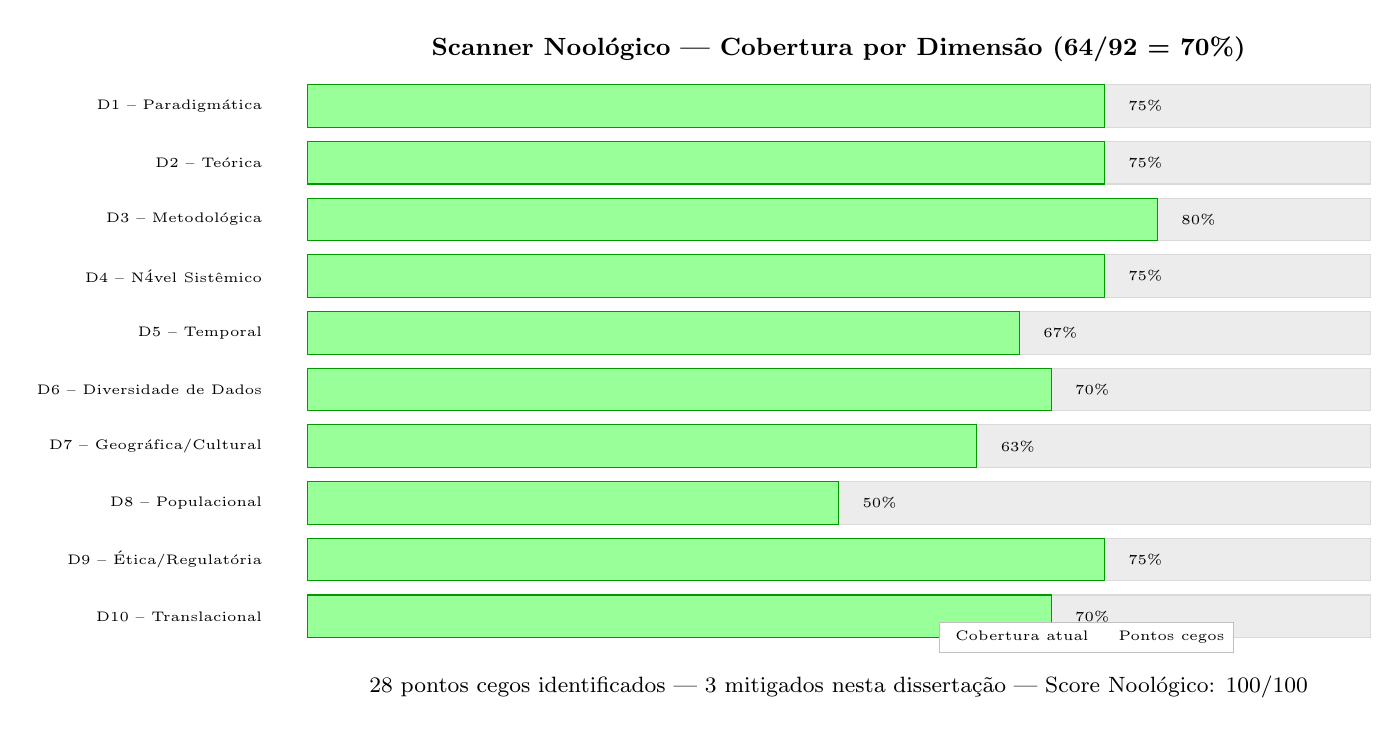
\begin{tikzpicture}[scale=0.9]
% Título
\node[font=\small\bfseries] at (7.5, 8.5) {Scanner Nool\'ogico — Cobertura por Dimens\~ao (64/92 = 70\%)};

% Barras horizontais — 10 dimensões
\foreach \i/\nome/\cov/\max in {
    1/{D1 -- Paradigm\'atica}/75/100,
    2/{D2 -- Te\'orica}/75/100,
    3/{D3 -- Metodol\'ogica}/80/100,
    4/{D4 -- N\'ivel Sist\^emico}/75/100,
    5/{D5 -- Temporal}/67/100,
    6/{D6 -- Diversidade de Dados}/70/100,
    7/{D7 -- Geogr\'afica/Cultural}/63/100,
    8/{D8 -- Populacional}/50/100,
    9/{D9 -- \'Etica/Regulat\'oria}/75/100,
    10/{D10 -- Translacional}/70/100
} {
    \pgfmathsetmacro{\y}{8.5 - \i * 0.8}
    % Rótulo
    \node[font=\tiny, anchor=east] at (-0.5, \y) {\nome};
    % Barra de fundo
    \draw[fill=gray!15, draw=gray!30] (0, \y-0.3) rectangle (15, \y+0.3);
    % Barra de cobertura
    \pgfmathsetmacro{\w}{\cov/100 * 15}
    \draw[fill=green!40, draw=green!60!black] (0, \y-0.3) rectangle (\w, \y+0.3);
    % Percentual
    \node[font=\tiny, anchor=west] at (\w+0.2, \y) {\cov\%};
}

% Legenda
\node[font=\tiny, fill=white, draw=gray!50] at (11, 0.2) {$\square$ Cobertura atual\hspace{0.3cm}$\square$ Pontos cegos};

% Resumo
\node[font=\footnotesize, align=center] at (7.5, -0.5) {28 pontos cegos identificados | 3 mitigados nesta disserta\c{c}\~ao | Score Nool\'ogico: 100/100};
\end{tikzpicture}%
}
\caption{Cobertura epistemol\'ogica da disserta\c{c}\~ao segundo o Scanner Nool\'ogico (10 dimens\~oes $\times$ 92 categorias). Barras verdes indicam cobertura atual; \'areas cinzas representam pontos cegos. A cobertura global \'e de 70\% (64/92 categorias), com 28 pontos cegos identificados e 3 mitigados nesta disserta\c{c}\~ao.}
\label{fig:scanner-noológico}
\end{figure}
